\section{Introduction}
\subsection{Problem Statement}
Cyclists, skateboarders, and scooter riders often face challenges in signaling their intentions to drivers, especially in low-light conditions. According to the CDC, 1,000 cyclists die and 130,000 are injured every year on the road in the United States (cite here). These numbers don’t include other riders sharing the road on things like skateboards and scooters. There are many interventions in place to prevent these accidents, such as fluorescent or retro-reflective clothing, or active lighting on the bicycle (required by law in most states) (cite here), but the traditional method of using hand signals is not always visible or practical, particularly at night or during adverse weather conditions. This lack of clear communication can lead to dangerous situations on the road, as other motorists may fail to recognize the cyclist's intended maneuvers, or if an accident occurs. 

\subsection{Proposed Solution}
To address this issue, we propose the development of a gesture recognition-based turn signaling system for cyclists and scooter riders. This system will utilize IMUs containing 9 degrees of freedom (3-axis accelerometer, 3-axis gyroscope, 3-axis magnetometer), integrated into a jacket. Then the data from the sensors will be processed to identify the specific arm gesture made by the rider and activate corresponding LED signals. For example, if the rider extends their arm straight to the left, the left turn signal is activated, or if the rider indicates a stop (arm out and forearm down), then the brake light is activated, and so on. Additionally, the sensors will be able to detect when the rider has had an accident or a crash, and activate a hazard signal on the LEDs.

We propose placing an IMU below the on the left wrist, and another on the waist. The microprocessor will then receive and process the data from the IMU, and determine what kind of movement has been made in real time. Then, depending on the movement, it will output a specific signal to the LEDs to display on the front and back of the wearable.

The final product achieved all 3 high level requirements. The device is able to correctly detect predefined arm gestures (raising right/left arm for turn signals, forearm down for slowing down) with an accuracy of 90\%. In addition, the device is able to correctly map the arm gestures into the different indications on the LEDs. The turn signal will be indicated by either the left or right side LED flashing red, while the brake/slow down signal will be indicated by all LEDs turning red. A crash or accident activates the hazard light, indicated by all LEDs flashing red. Lastly, the turn signals, brake lights, and hazard signals were all visible and easily identifiable from a distance of at least 250 feet to ensure that they are clearly visible at both day and night. All of these functionalities ensure that hand gestures are more visible to drivers and other people, thereby increasing the safety of the rider.
\newpage

\subsection{Visual Aid}
Figure \ref{fig:vis_aid} is a mockup of the wearable device that we created. The device will be powered by a battery and will have 2 IMUs to detect the arm gestures. The system will be controlled by an ESP-32 microcontroller that will process the data from the IMUs and send a signal to the LEDs to turn on when the arm gestures are detected.
\begin{figure}[ht]
    \centering
    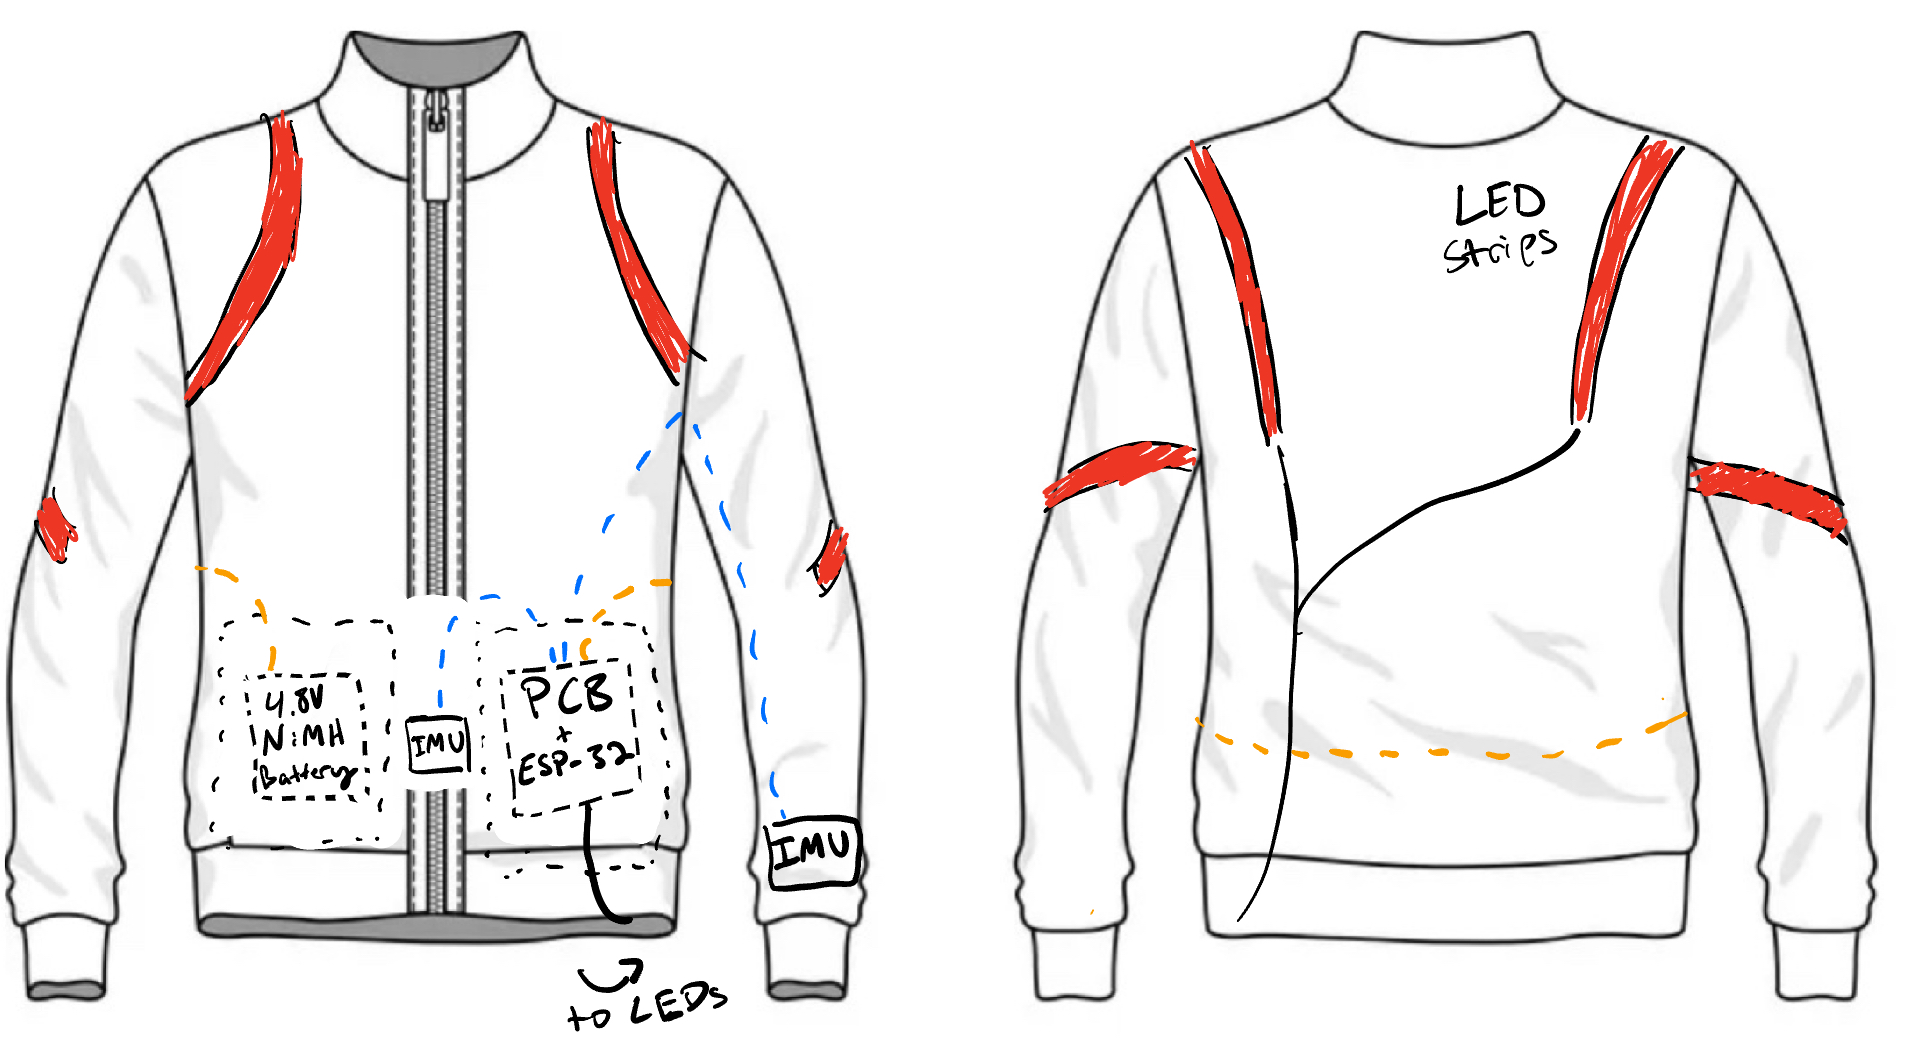
\includegraphics[width=0.8\textwidth]{images/visual_aid_new.jpg}
    \caption{Visual Aid mockup of the wearable \cite{VectorStock2024}}
    \label{fig:vis_aid}
\end{figure}

\subsection{Block Diagram}
\begin{figure}[ht]
    \centering
    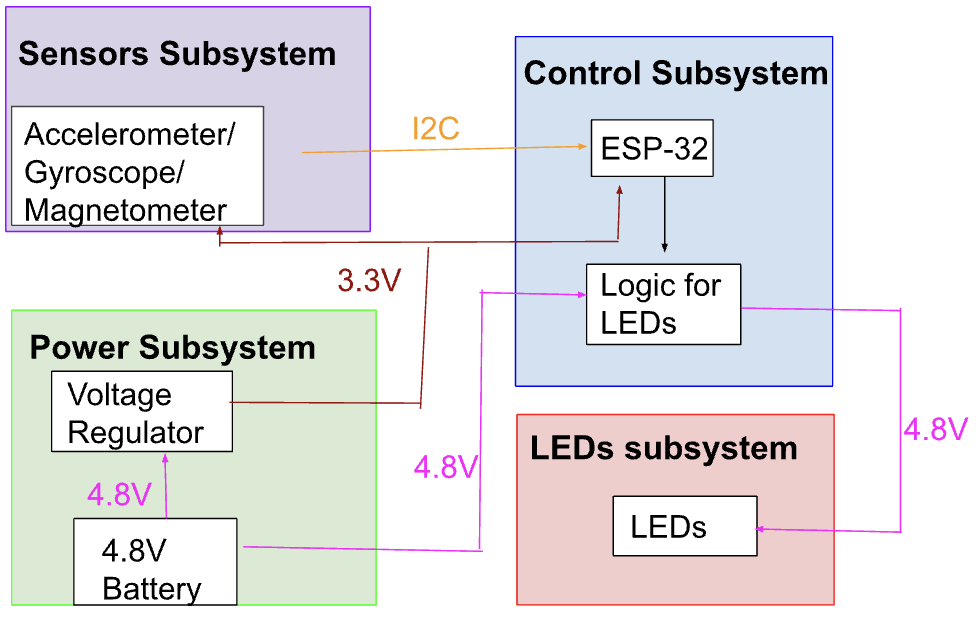
\includegraphics[width=0.8\textwidth]{images/block_diagram_new.png}
    \caption{Block Diagram of the system}
    \label{fig:block_diagram}
\end{figure}
As can be seen from the block diagram in figure \ref{fig:block_diagram}, the device is split into 4 subsystems: Sensors, Control, Power, and LEDs. The power subsystem provides 4.8V to the LEDs through a BJT that gets a signal from the ESP-32. The Control Subsystem and the Sensor Subsystem receive 3.3 volts from the battery through a voltage regulator. The Control Subsystem receives real-time data from the 2 IMUs through I2C, processes the data, then sends a signal to the gate to turn the LEDs on when the IMU data is within a certain range.


\newpage
